\chapter{Avoiding Burnout: Energy, Sales, and the Word No}

This short interview segment begins with a practical question and answers it with a compact operating model. Burnout is treated not as a mysterious state but as the result of failing to control energy and emotion. The speaker then turns that claim into a daily budget: we begin with a finite reserve, spend it through communications, interactions, and decisions, and protect it by refusing work that does not add value to ourselves, the business, or the team.

\section{The Opening Question}

The interview opens directly: how do we avoid burnout, and what keeps us motivated? The important feature of the question is that it combines two things that are often separated. Burnout is a depletion problem; motivation is a continuation problem. The answer given in the lecture treats both through the same lens: control the expenditure of internal resources.

\subsection{Question \& Answer}

\paragraph{Question.}
How do we avoid burnout, and what keeps us motivated?

\paragraph{Answer.}
The speaker's answer is that burnout happens when we fail to control energy and emotion. The point is not presented as a clinical theory. It is an operator's rule: if energy and emotional response are allowed to be spent by every request, every conversation, and every decision, the day consumes the person before the person can direct the day.

\section{Burnout As A Control Problem}

The first move is definitional. Burnout is connected to a loss of control over two resources:
\begin{itemize}
\item energy, the finite capacity to act, decide, and respond;
\item emotion, the internal state that determines how costly each interaction feels.
\end{itemize}

We can write this only as a bookkeeping analogy, not as a formula from the interview. Let
\[
E_0
\]
denote the usable energy with which a person begins the day. The speaker's claim is that this starting quantity is finite. It may vary from person to person and from day to day, but in the logic of the lecture it is never infinite.

If \(E_{\mathrm{remain}}\) is the energy left after the day's demands, then the simplest reconstructed model is
\begin{equation}
E_{\mathrm{remain}} = E_0 - \sum_i c_i ,
\end{equation}
where \(c_i\) is the cost of one communication, interaction, or decision. The equation is not a measurement system. It is a disciplined way of preserving the spoken mechanism: small drains accumulate.

\section{The Daily Energy Budget}

The next step in the lecture is the daily-budget picture. We wake up with a certain amount of energy. Then the day begins to draw it down. The speaker names three sources of drain in sequence: communication, interaction, and decision.

A slightly more explicit reconstruction separates those categories:
\begin{equation}
E_{\mathrm{remain}}
=
E_0
-
\sum_j C_j
-
\sum_k I_k
-
\sum_{\ell} D_{\ell}.
\end{equation}

Here \(C_j\) denotes the cost of communication \(j\), \(I_k\) the cost of interaction \(k\), and \(D_{\ell}\) the cost of decision \(\ell\). The notation should stay modest. Its job is to keep the lecture's rhythm clear: one small expenditure is not the whole story; repetition is the whole story.

\begin{figure}
\centering
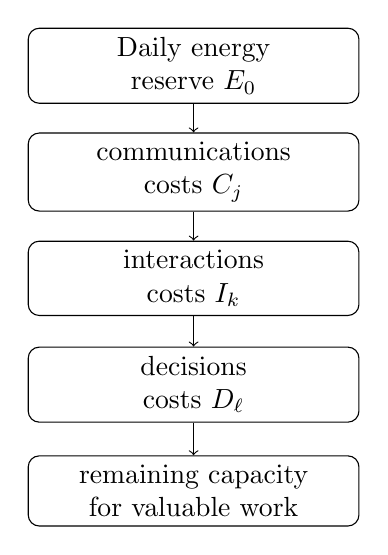
\begin{tikzpicture}[x=1cm,y=1cm]
\node[draw, rounded corners, align=center, minimum width=4.2cm, minimum height=0.75cm] (start) at (0,0) {Daily energy\\reserve \(E_0\)};
\node[draw, rounded corners, align=center, minimum width=4.2cm, minimum height=0.75cm] (comm) at (0,-1.35) {communications\\costs \(C_j\)};
\node[draw, rounded corners, align=center, minimum width=4.2cm, minimum height=0.75cm] (inter) at (0,-2.70) {interactions\\costs \(I_k\)};
\node[draw, rounded corners, align=center, minimum width=4.2cm, minimum height=0.75cm] (dec) at (0,-4.05) {decisions\\costs \(D_{\ell}\)};
\node[draw, rounded corners, align=center, minimum width=4.2cm, minimum height=0.75cm] (remain) at (0,-5.40) {remaining capacity\\for valuable work};

\draw[->] (start) -- (comm);
\draw[->] (comm) -- (inter);
\draw[->] (inter) -- (dec);
\draw[->] (dec) -- (remain);
\end{tikzpicture}
\caption{A transcript-derived reconstruction of the daily energy budget. No board diagram was available; the figure summarizes the lecture's spoken mechanism.}
\end{figure}

\section{Why Sales Makes The Drain Stronger}

After the energy model is introduced, the lecture pivots into entrepreneurship. The speaker widens the audience: a business owner, a company leader, a person in real estate, or really anyone trying to operate commercially is in sales.

The claim is not that every person holds a sales title. The claim is that every interaction has a sales-like structure. We are asking for attention, granting attention, persuading, judging, responding, and deciding whether the exchange is worth the cost. That is why the energy budget matters more, not less, in business.

Let \(r\) denote an incoming request, conversation, opportunity, or demand on attention. Let \(c(r)\) be the cost of engaging with it, and let \(V(r)\) be the value it adds to the person, the business, or the team. The lecture's practical test can be reconstructed as
\begin{equation}
\mathrm{Engage}(r)=1
\quad \Longleftrightarrow \quad
V(r) > c(r).
\end{equation}

The opposite case is the rule that the speaker emphasizes:
\begin{equation}
\mathrm{Decline}(r)=1
\quad \Longleftrightarrow \quad
V(r) \leq c(r).
\end{equation}

Again, this is not a literal formula from the interview. It is the cleanest mathematical version of the phrase ``worth your time.''

\section{The Rule Of No}

The conclusion of the lecture is practical: the word no becomes more important. In the energy-budget picture, no is not merely a boundary. It is an allocation rule. It prevents low-value demands from consuming the reserve needed for higher-value work.

A short worked example makes the logic concrete. Suppose a day begins with
\[
E_0 = 100
\]
units of usable energy. The units are artificial, but the arithmetic follows the lecture's claim. Suppose the day contains communications, interactions, and decisions with total costs
\[
\sum_j C_j = 20,
\qquad
\sum_k I_k = 35,
\qquad
\sum_{\ell} D_{\ell} = 25.
\]
Then
\begin{align}
E_{\mathrm{remain}}
&=
100 - 20 - 35 - 25 \\
&=
20.
\end{align}

Now suppose an additional interaction \(r\) costs \(c(r)=15\). If it adds only \(V(r)=5\) units of value to the person, the business, or the team, then
\[
V(r) < c(r),
\]
so the reconstructed rule says to decline it. The reason is not that interaction is bad. The reason is that an interaction with low value and high cost would reduce the remaining reserve from \(20\) to \(5\), leaving little capacity for work that actually matters.

In this sense, saying no is not avoidance. It is conservation for the sake of execution.

\section{A Cautious Burnout Threshold}

The lecture does not give a diagnostic threshold for burnout, and we should not invent one. But its logic points to a qualitative danger condition:
\begin{equation}
\sum_i c_i \gg E_0.
\end{equation}

Read this only as a warning sign. If the accumulated cost of communications, interactions, and decisions greatly exceeds the controlled daily reserve, the operator is no longer choosing where energy goes. The day is choosing for him.

The role of emotional control is also important here. Two identical interactions may not have identical costs. An interaction handled with control may have cost \(c_i\); the same interaction handled reactively may have a larger cost. In symbols, we might write
\begin{equation}
c_i^{\mathrm{reactive}} > c_i^{\mathrm{controlled}},
\end{equation}
as a cautious reconstruction of the speaker's link between emotion and burnout.

\section{Summary}

The segment moves in a tight order. It begins with the question of burnout and motivation, answers by naming energy and emotional control, develops a daily reserve model, then applies that model to business, leadership, real estate, and sales. The final rule is simple but not shallow: every interaction consumes capacity, so each interaction must be tested for value. The word no protects the energy needed for the work that adds value to the person, the business, and the team.